\section{Konditionerings apparat}
Konditioneringsapparatet er opbygget af flere blokke, som kan ses på figur \ref{fig:BDD(SystemOverview)}. Blok difinition diagrammer beskriver relationerne mellem blokke, så som sammenhæng, forening og specialisering. I denne sammenhæng beskriver figur \ref{fig:BDD(SystemOverview)} opbygningen af konditioneringsapparatet. 
\begin{figure}[H]
	\centering
	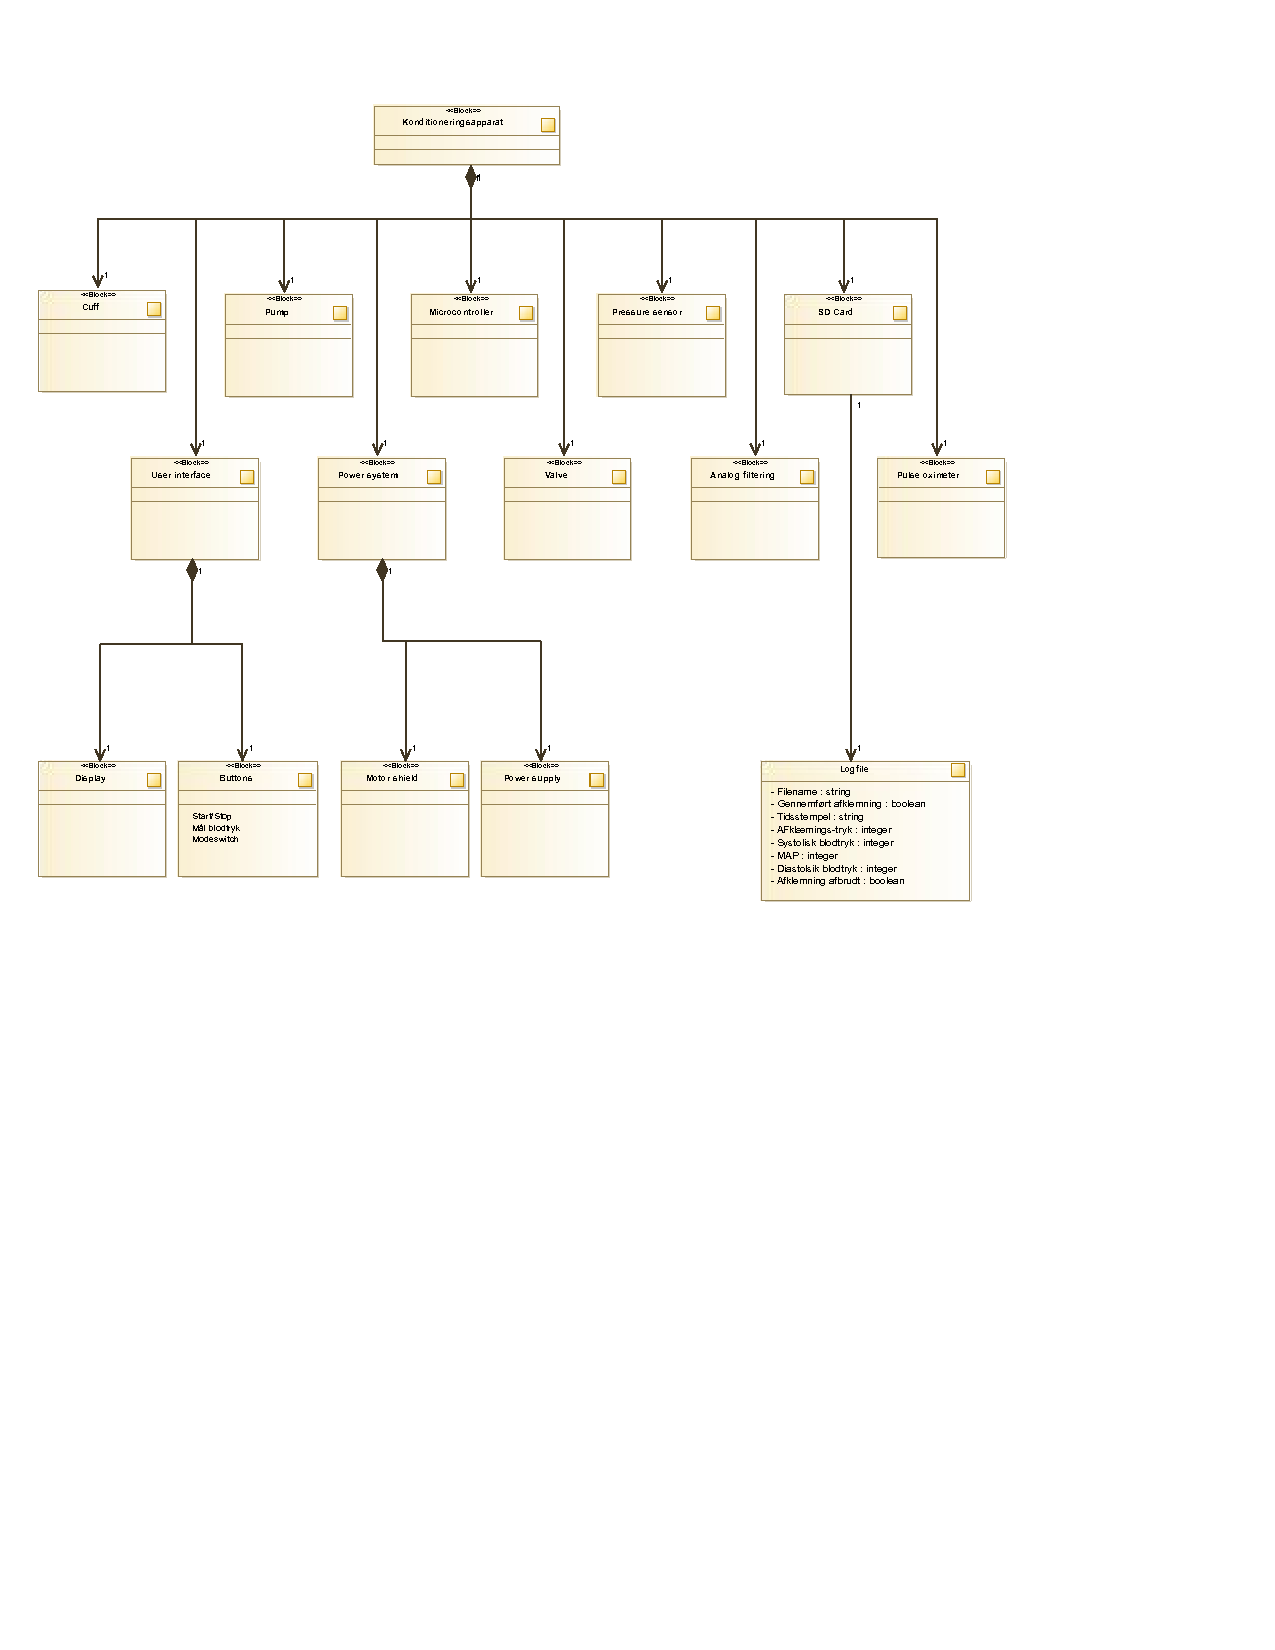
\includegraphics[width=0.9\textwidth]{billeder/BDD(SystemOverview).pdf}
	\caption{Block difinition diagram over konditioneringsapparatet.}\label{fig:BDD(SystemOverview)}
\end{figure}

\subsection{Oscilumetrisk blodtryks apparat}
Den oscillometriske blodtryks måle metode, beskrevet i afsnit \ref{noninvasivBloodpressureMeasurement}, blev implementeret som beskrevet i implementeringsdokumentet\fixme{reff: implementeringsdokument} og resultaterne der af er beskrevet følgende.

Det pulserende signal fra tryksensoren, som blodtryksmåleren analyserer er i sin rå (ubehandlet) tilstand støjfyldt. Signalet beskrevet i afsnit \ref{noninvasivBloodpressureMeasurement} på figur \ref{fig:OscillometriskMetode} er meget rent og amplitude højderne danner en flot parabel kurve. På figur \ref{fig:rawPulseSignal} ser det pulserende signal indhyldet i støj. Kurven er stødt faldende, fordi trykket i manchetten langsomt lukkes ud. Ydermere observeres der også varierende amplitudehøjder, som ikke er stødt stigende/faldende, men virker  tilfældigheder.  

\begin{figure}[H]
	\centering
	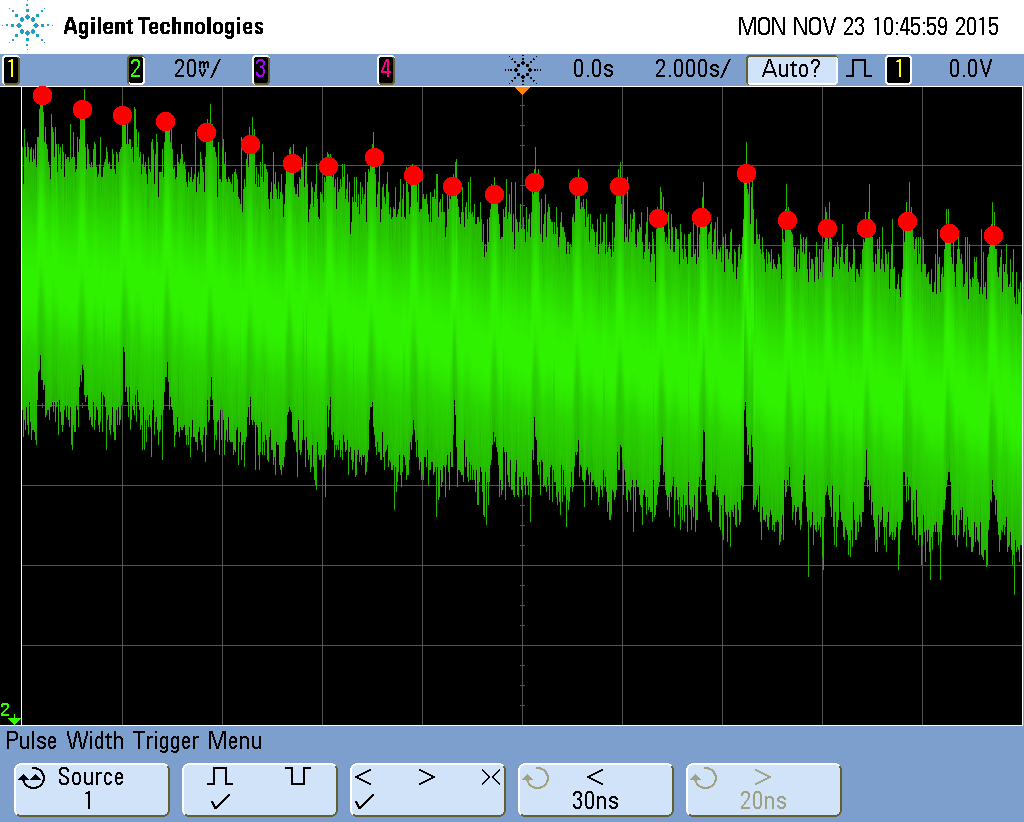
\includegraphics[trim={0 7cm 0 1.5cm},clip, width=1\textwidth]{billeder/rawPulseSignalPeaks.png}
	\caption{Osclilloskops måling af rå signal fra blodtryksmåling, med konditioneringsapparatet. De røde cirkler er pulse oscillotionernes højeste punkt}\label{fig:rawPulseSignal}
\end{figure}

Efter analog filtrering af det rå signal ved en endnu en blodtryksmåling med konditioneringsapparatet, ses at amplitude oscillotionerne isoleret og uden manchet trykket. Over en hel blodtryksmåling viser kurven beskrevet i teorien (figur \ref{fig:OscillometriskMetode}) sig, med en stigende amplitudehøjde efterfulgt af en top og til sidst en faldende oscillotionshøjder med laverer hældnings koefficient. En hel blodtryksmåling med filtreret råsignal kan ses på figur \ref{fig:filteredPulseSignal}.

\begin{figure}[H]
	\centering
	\subbottom[Stigende]{%
		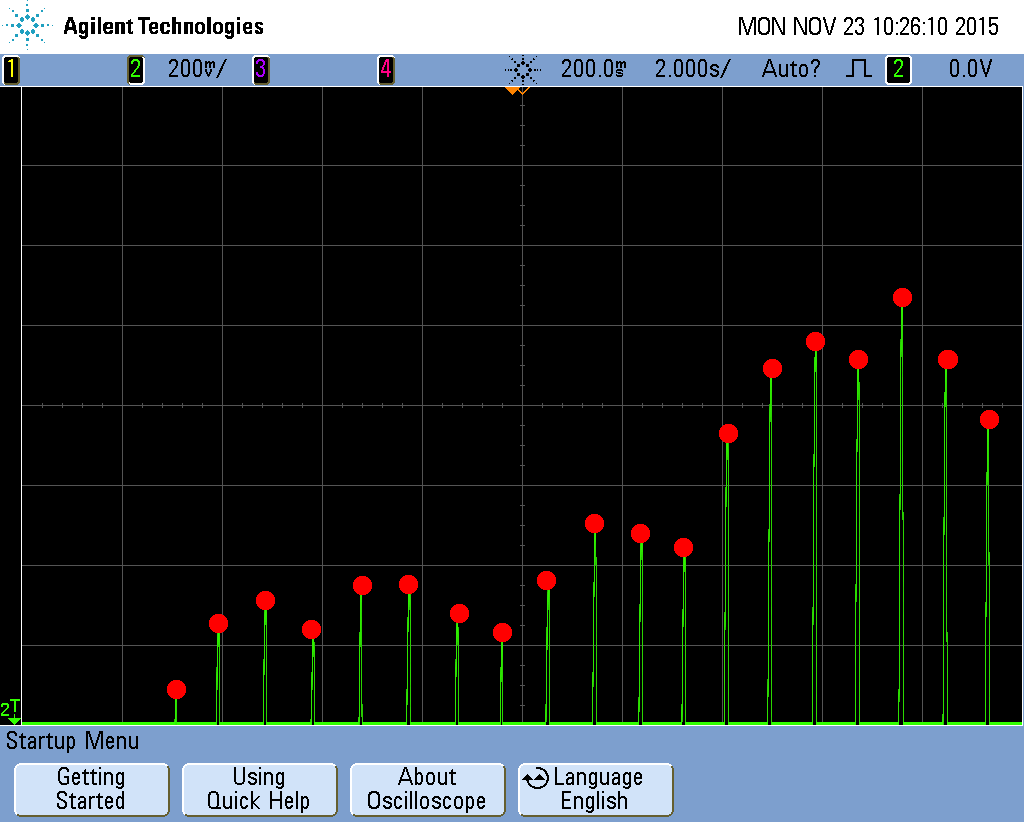
\includegraphics[trim={0 3.3cm 0 1.5cm},clip, width=0.328\textwidth]{billeder/filteredPulseSignalPeaks1.png}}
	\subbottom[Højdepunkt]{%
		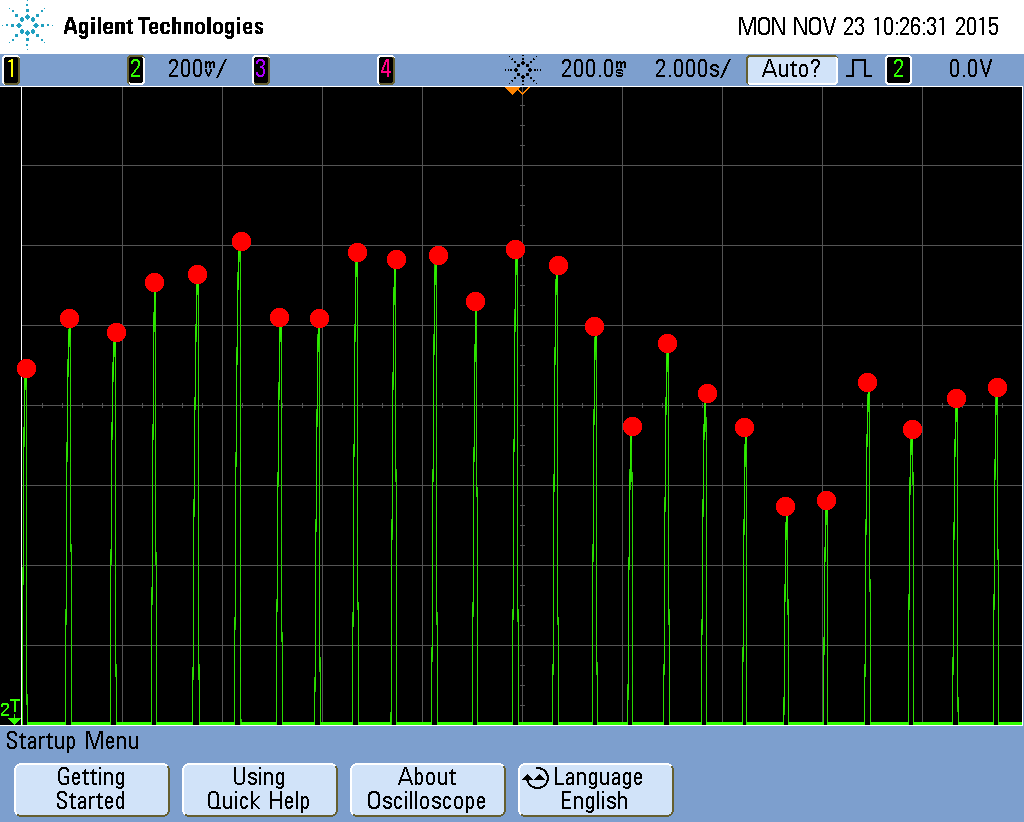
\includegraphics[trim={0 3.3cm 0 1.5cm},clip, width=0.328\textwidth]{billeder/filteredPulseSignalPeaks2.png}}
	\subbottom[Faldende]{%
		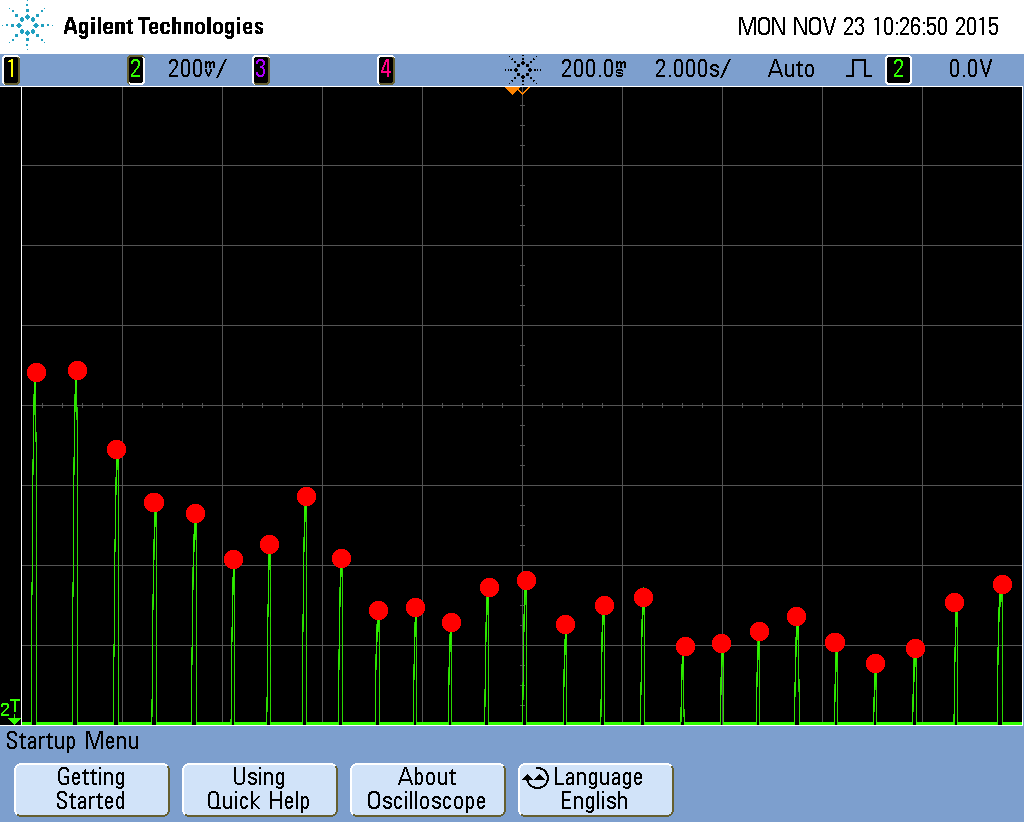
\includegraphics[trim={0 3.3cm 0 1.5cm},clip, width=0.328\textwidth]{billeder/filteredPulseSignalPeaks3.png}}
	\caption{Osclilloskops måling af filtreret signal af blodtryksmåling, med konditioneringsapparatet. (a) er første del af blodtryksmålingen, (b) er de midten af signalet med, hvor MAP befinder sig og (c) er slutningen af signalet, hvor amplituderne flader ud. De røde cirkler er pulse oscillotionernes højeste punkt}\label{fig:filteredPulseSignal}
\end{figure}

\subsubsection{Analog filtrering}
Den analoge filtrerings som ses på forskellen mellem figur \ref{fig:rawPulseSignal} og figur \ref{fig:filteredPulseSignal} er implementeret i implementeringsdokumentet se \fixme{ref: implementeringsdokument}. 
Det resulterende analoge filter, bestemt ud fra test opsætninger (se \fixme{ref: implementeringsdokument}) og litteraturen \fixme{CHARACTERIZATION OF THE OSClLLOMETRlC METHOD FOR MEASURING INDIRECT BLOOD PRESSURE}, er de pulserende oscillationer isoleret til et pulserende signal, som kan ses på figur \ref*{fig:filteredPulseSignalWithFFT}. Resultatet er opnået, ved at implementerer et båndpasfilter, med et pasbånd som starter før lavest mulig puls og slutter ved den tiende afledte af grundfrekvensen 60bmp (se figur \ref*{fig:BandPassFilter}).

\begin{figure}[H]
	\centering
	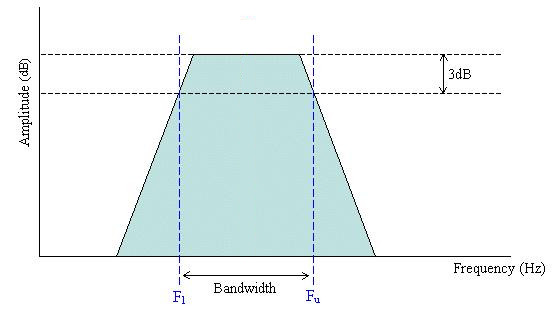
\includegraphics[trim={0 0 0 1.5cm},clip, width=0.8\textwidth]{billeder/BandPass_filter.JPG}
	\caption{Bånd pass filter med passfilter mellem $F_1$ og $F_u$. $F_1=0.22Hz$ (13 bmp under mulig puls) og $F_u=11Hz$ (660 bmp 10 afledte af 60 bpm) }\label{fig:BandPassFilter}
\end{figure}

\begin{figure}[H]
	\centering
	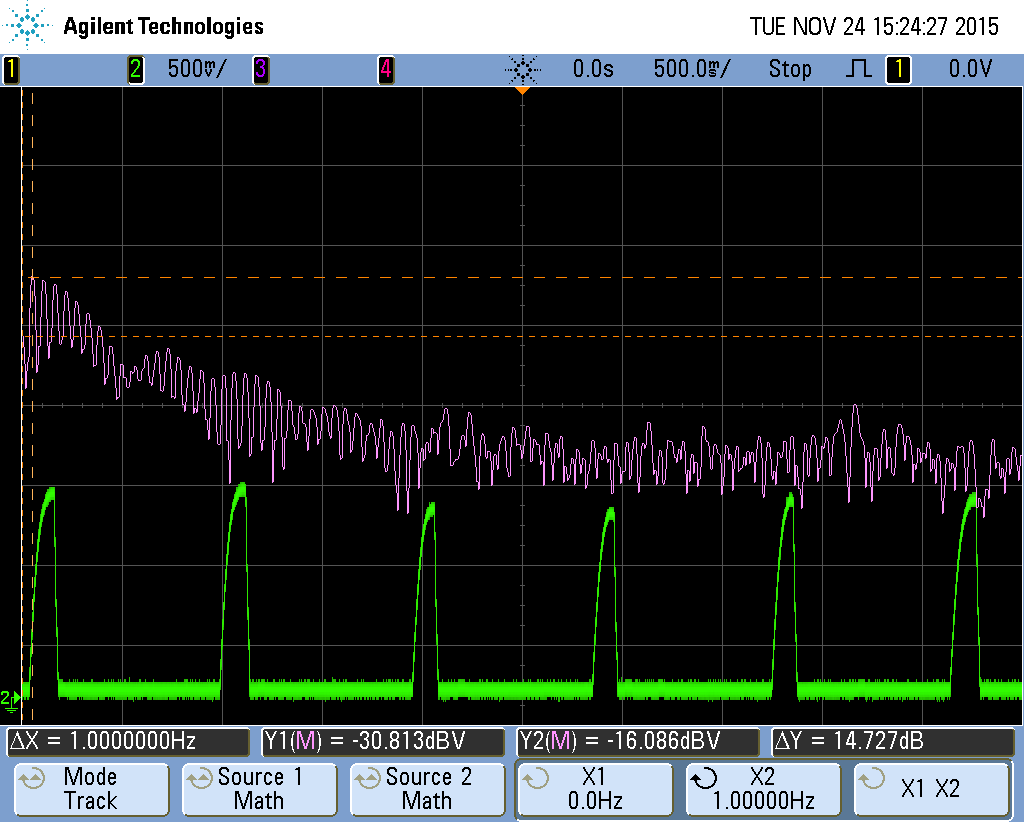
\includegraphics[trim={0 0 0 1.5cm},clip, width=1\textwidth]{billeder/filteredPulseSignalWithFFT.png}
	\caption{Osclilloskops måling af filtreret signal fra manchetten oppustet på arm. den røde kuve er de pulserende oscillotioner og den lyserøde kurve er en Fast Fourier Transformation (FFT) af den røde kurve, hvor den udregnede grundfrekvens af oscillationerne måles til 1Hz (60 bpm).}\label{fig:filteredPulseSignalWithFFT}
\end{figure}

\subsubsection{Digital filtrering}
For at opnå en glat parappel, som vist på  figur \ref{fig:OscillometriskMetode}, er der implementeret et digitalt filter, som har til opgave at udglatte oscillutions amplituderne fra blodtryksmålingerne. Resultatet af implementeringen kan ses på figur \ref{fig:digitalFilterData}. Det bedste forhold mellem udglatning og reaktionshastighed af filteret blev opnået med et ekspotentielt filter $y(n)=\alpha*x(n)+(1-\alpha)*y(n-1)$

\begin{figure}[H]
	\centering
	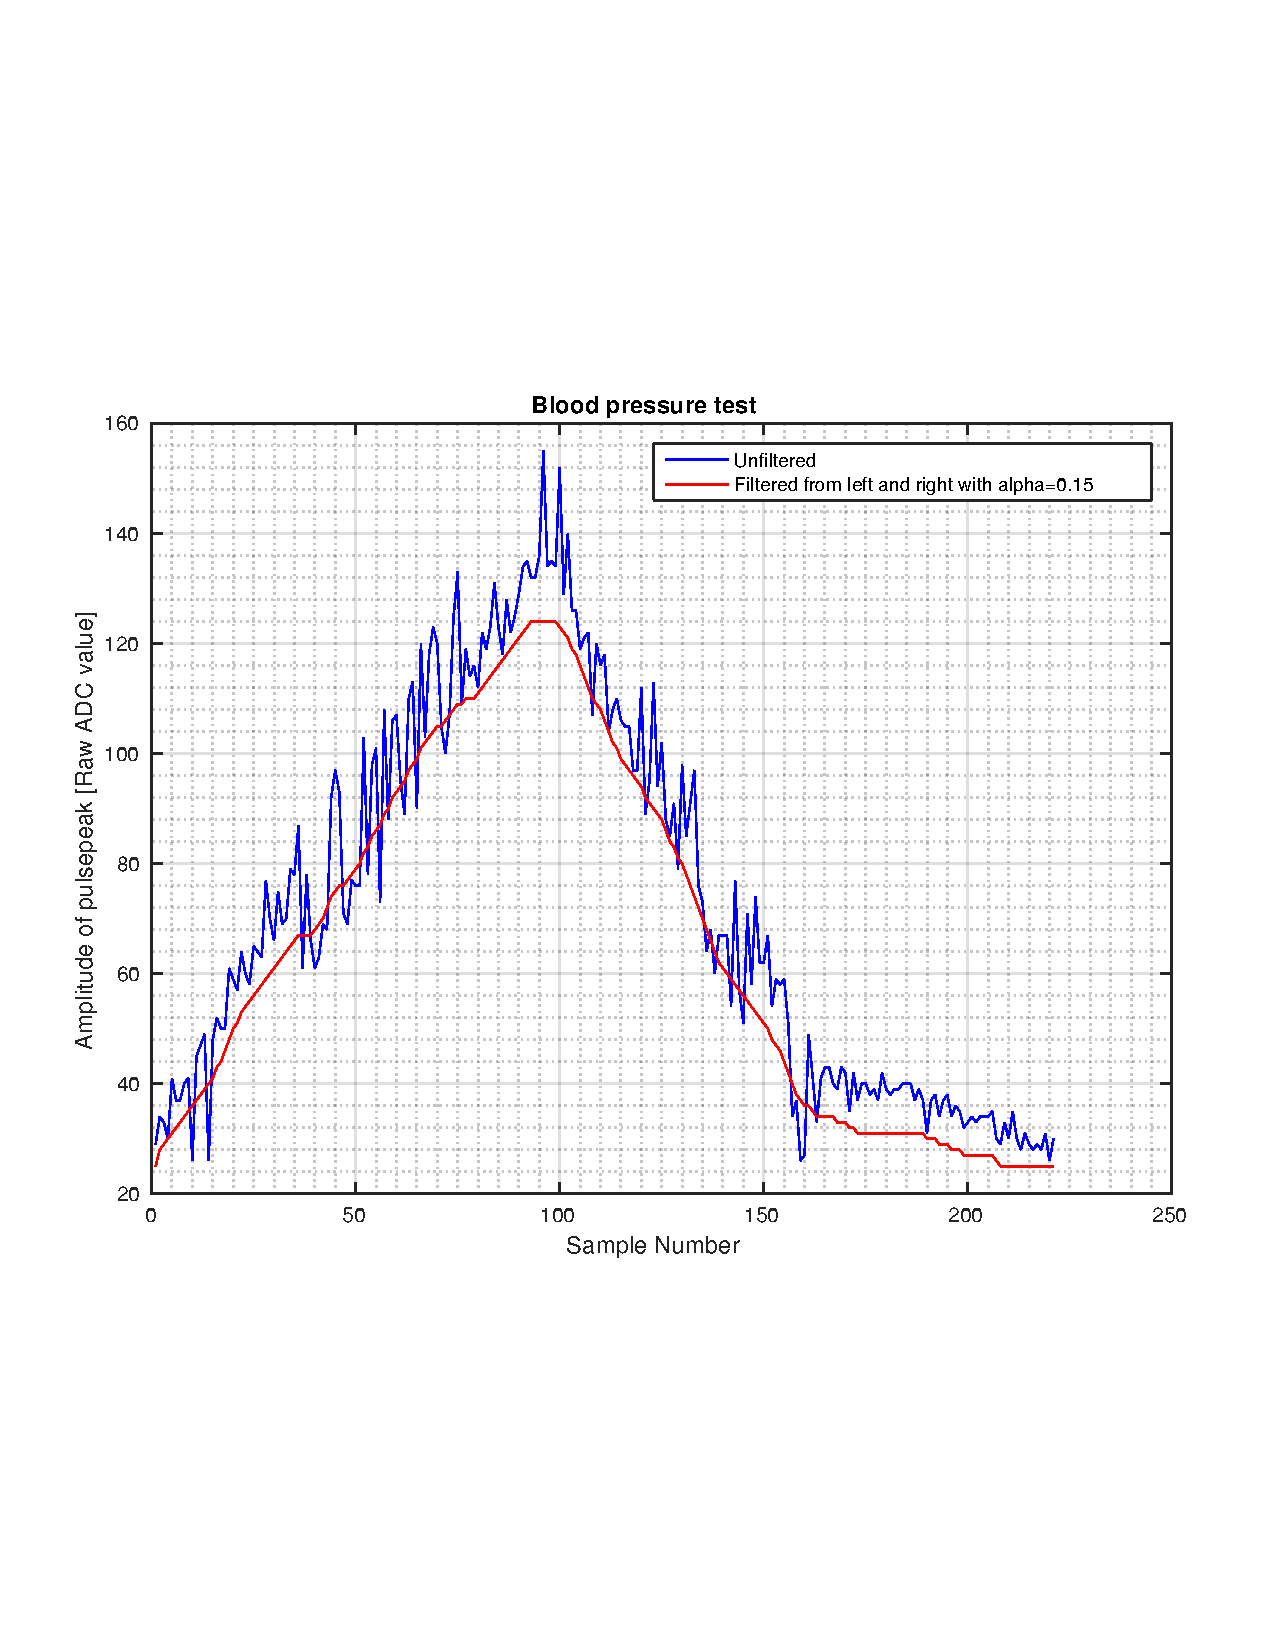
\includegraphics[trim={0 0 0 0},clip, width=0.7\textwidth]{billeder/digitalFilterData.pdf}	
	\parbox{10.5cm}{\caption{Digital filtrering af oscillotions peaks fra blodtryksmåling på simulator med ekspotentiel midlingsfilter.}\label{fig:digitalFilterData}}
\end{figure}


\subsection{Fikseret-ratio} \label{Fikseret-ratio}